\documentclass[11pt,twocolumn]{jarticle} %11pt が MS-Word の10.5pt 相当
\usepackage[a4paper,left=23mm,right=23mm,top=27mm,bottom=32mm]{geometry} 

\usepackage[dvipdfmx]{graphicx}
\usepackage{iit-en-sjis} %use iit-en-sjis if the body text is written English.
\usepackage{wrapfig}
\usepackage{algorithm, algpseudocode}
\usepackage{algorithmicx}
\usepackage{comment}
\usepackage{amsfonts}

\graphicspath{ {imgs/} }

\title{捕食者・獲物環境におけるマルチエージェントの分散型協調学習}
\etitle{Distributed Multi-Agent Cooperation Learning in Predator-Prey Environment}

\author{唐 \ \ 霄}
\eauthor{TANG Xiao}

\advisors{
\footnotesize
\begin{tabular}{ll}
 指導教員: & 延原 肇, 中内 靖, 星野 准一(知能機能工学域)\\
\end{tabular}
}
\eadvisors{
\scriptsize
\begin{tabular}{ll}
Supervised by: & Nobuhara Hajime, Yasushi Nakauchi and Junichi Hoshino (Division of Intelligent Interaction Technologies) \\
\end{tabular}
}

\authorheader{唐 \ 霄}
% use English name when you use the English style

\dateheader{2018年3月}

\abstract{
(Remain modification)
Research of Moving Target Search is ongoing recent years. There are some researches according to the problem of Multi-Agent pursuing a moving target, but few of them could be applied to real world. This research focused on this problem and proposed a speed-up method for real-time grid environment based on Cover Heuristic method. We use Map Abstraction to build map hierarchy which helps us do faster map search compared to previous method. Refinement is used for highly-abstracted route refining to successor original map. Finally, evaluation experiments are based on Benchmark maps and the result showed high efficiency of our proposed method.
}

\keywords{keyword-1, keyword-2, keyword-3, keyword-4, keyword-5, keyword-6}

\begin{document}

\maketitle
\thispagestyle{iitheader}
\section{Introduction}
Recently, AI arouse hot topics around the world, especially the appearence of AlphaGo\cite{alphago}. DeepMind introduced their Go player which is called AlphaGo in 2015, they beat several human being's top professional players of over the past two years. And AlphaGo evolved to higher version? which are AlphaGo Master and AlphaGo Zero\cite{alphagozero}. Not only the application to traditional sports, Game is also a big area which study are ongoing. DeepMind and Blizzard released StarCraft II as an AI research environment\cite{starcraft} to researchers around the world which could help human-being to have a better acknowledge of game strategy.\par

\begin{figure}[t]
 \begin{center}
  \includegraphics[width=5cm]{imgs/adversary_chasing.png}
  \caption{Predator-Prey}\label{fig:adversaryChasing}
 \end{center}
\end{figure}

Deep Reinforcement Learning (DRL) is one of the technologies which support AI development. There are a lot of applications from game playing\cite{game} to robot controlling\cite{robot}. Also, Google applied Deep Learning to data center coolinng by 40\%\cite{google} electric cost off. Healthcare and finance are the areas which are being researched and expected to have a greate impact to sociaty. However, despite the fact that DRL is successfully applied to many single-agent domain tasks, there are varianty of applications which are in multi-agent domain. These application needs multiple agents to evolve together resulting in good communication or cooperation. For instance, multi-character controlling in game playing, multi-agent system in delivery system and so on.


One representative for multi-agent task is Predator-Prey\cite{maddpg}, showed in Figure \label{fig:adversaryChasing}. In above case, there are 3 predators, 1 prey and 2 landmarks (obstacles) in this map. Predators move with slower speed compared to prey to chase the faster moving prey. For human being, the cooperation strategy of splitting up and surrounding is absolutely easy to understand and learn. Unfortunately, it is difficult for agent to learn. Although Traditional reinforcement learning such as Q-learning\cite{qlearning}, Policy Gradient\cite{pg} performs greatly or even over human being in Atari Game\cite{ddpg}, it performs poorly in multi-agent domain. The reason why the successful RL methods using in single-agent domains could not acquire the same result in multi-agent domain is that along with mult-agent self-learning, the environment becomes non-stationary which failed in convergence. \par

(Remain modification)
In this work, we first introduce several prior work and related researches and why they failed in multi-agent domain. Then we will explain our proposed method - Distributed Multi-Agent Cooperation Algorithm besed on MADDPG algorithm\cite{maddpg}. Our method includes the multiple workers distributly working on each thread and the learning rate tuning using Proximal Policy Optimization\cite{ppo}. \par

Evaluation experiments shows our method performed better than MADDPG and traditional Deep Reinforcement Learning method DDPG. \par

\section{Background} 
In this section, we introduce several related researches and discuss why they cannot be applied to multi-agent domain task.
\subsection{Cover-hueristic Algorithm}
As for prior research for solving Predator-Prey, I have proposed a cooperation searching algorithm\cite{cover} towards this task. This method is based on map search using cover-heuristic (maxmizing Predator's moving area and minimizing prey's moving area) and accelarate search by map abstraction and refinement. However, this method performs well in small-size maps but poorly in big-size maps, the computational time is depends on the map size. A agent which could be called intelligent should have its own mind like human beings. This kind of AI is able to take actions based one its own policy.\par


\subsection{Reinforcement Learning and Multi-Agent Markov Decision Process}

Reinforcement Learning (RL) is method that agent learns to make decisions through interaction with the environment. An agent interacts with environment and becomes able to alter its behaviour according to the reward it recieved from environment along with observing the consequences of its actions. \par

In RL settings, agent is controlled by specific algorithm (machine learning). At timestep $t$, the agent observes a state $s_t$ which describes possible configurations of all agents in environment and interacts with it by taking an action $a_t$. After agent takes an action, the environment and agent transition to a new state $s_{t+1}$. The state represents sufficient necessary information which could have agent's informations (position, velocity) and other environment information. Each time the environment transitions to a new state, agent recieves an reward $r_t$ as feedback. The goal of the agent is to learn a policy $\pi$ which maximizes the expected cumulative reward. However, the challenge in RL is that agent needs to learn about the consequences of actions by trail and error instead of one step action. The action-learning loop is illustrated in Figure \ref{fig:rl}. \par
\begin{figure}[h]
 \begin{center}
  \includegraphics[width=8cm]{imgs/RL.PNG}
  \caption{
  The Agent-Action-Learning loop. At time $t$, the agent recieves state $s_t$ from the environment. The agent uses its policy $\pi$ to choose an action $a_t$. Once the action is executed, the environment transitions a step, providing the next state $s_{t+1}$ as well as feedback in the form of a reward $r_{t+1}$. The agent uses knowledge of state transitions, of the form ($s_t$, $a_t$, $r_{t+1}$, $s_{t+1}$), in order to learn and improve its policy.
  }
  \label{fig:rl}
 \end{center}
\end{figure}

The RL could be described as a Markov Decision Process (MDP). in our work, we extend MDP from single agent domain to multi-agent setting. The multi-agent MDP consists of (timestep $t$ is omitted):
\begin{itemize}
  \item $n$ Agents.
  \item State $s$ which describes agents' configuration.
  \item A set of observations $o_1$, $o_2$ ... $o_i$ ... $o_n$ from state, $_i$ is agent's index.
  \item A set of actions $a_1$, $a_2$ ... $a_i$ ... $a_n$ chosen from each agent.
  \item Policy $\pi_i$ of agent $i$: \[\pi_i: o_i \rightarrow a_i\] which represents given the observation, agent uses its policy to choose an action.
  \item A set of rewards $r_1$, $r_2$ ... $r_i$ ... $r_n$, agents recieves rewards from environment after execution of their chosen actions.
\end{itemize}
Each agent is trying to maxmize its total expected reward, which could be represents as,
\[ \sum_{t=0}^{T-1}(\gamma^t r_i^{t+1}) \]
where $t$ is timestep and $T$ is the length of one episode, gamma is the discounted factor $\gamma$ $\subseteq$ $(0, 1]$

\section{Related Work}

Currently, there are three approaches to solve MDP problems: value-based method, policy-based method and actor-critic method. We will discuss these methods about their advantages and drawbacks in solve multi-agent domain problems.

\subsection{Value-based Method}

Value-based method is based on estimating the expected return of being given a state. The state-value function $V^\pi(s) = \mathbb{E}[R|s, \pi]$ is expected return when starts from state $s$ and following the policy $\pi$. When we have optimal policy, $\pi$ becomes $\pi^*$. \par
However, value function can not provide us transitions for agent to learn. Therefore, action-value function $Q^\pi(s, a)$ could help. Action-value function needs initial action $a$ input and state $s$, the following state is based on policy $\pi$. The best policy could be found by choosing maximal $Q$ value with action a which represents as $argmax_a Q^\pi(s, a)$. 

\subsubsection{Q-learning}

Q-learning is one of famous algorithms in RL. We update action-value function using a Bellman equation where t is timestep: 
\begin{equation}
Q^\pi(s_t, a_t) = \mathbb{E}_{s+1}[r_{t+1} + \gamma Q^\pi(s_{t+1}, \pi(s_{t+1}))].  
\end{equation}
\begin{equation}
Q^\pi(s_t, a_t) \leftarrow Q^\pi(s_t, a_t) + \alpha\delta.  
\end{equation}
where $\alpha$ is learning rate and $\delta = y - Q^\pi(s_t, a_t)$ is the Temporal Difference (TD) error; We can see that $Q^\pi$ can be improved by \textsl{bootstrapping}.\par 
Q-learning is an off-policy algorithm, because $Q^\pi$ is updated by transitions that were not generated by derived policy where $y = r_t + \gamma\max_a Q^\pi(s_{t+1}, a)$which is the approximation of $Q^*$.
\subsubsection{Deep Q-learning}

Deep Q-learning (DQN) \cite{dqn}  is the extended version of Q-learning using deep learning. It uses a deep neural network to work as the Q value function. 
\begin{equation}
L(\theta) = E_{s,a,r,s'}[(Q^*(s, a|\theta) - y)^2],  
\end{equation}
$$where\ y = r + \gamma\max \bar{Q}^*(s', a')$$

where $\theta$ is the parameters in neural network, $(s,a,r,s')$ is the transition we used. \par

This TD-loss shows in Equation 3. We could improve the estimate of Q-value function by minimizeing TD errors from trajectories which are experienced by following the policy. The optimization method is Stocastic Gradient Desecent (SGD), resulting in convergence of value function. \par
DQN has two important techniques to keep training process stable: experience and target networks.\par
Experience replay \cite{replay} memory stores transitions of the form $(s,a,r,s')$ , enabling the agent to sample from and train on previously observed data offline. By sampling from a large memory, the temporal correlations that could adversely affect RL algorithms are broken. [Whilst the original DQN algorithm used uniform sampling [84], later work showed that prioritising samples based on TD  rrors is more effective for learning [118].] \par
Target networks \cite{qlearning} is to maintain the weights of network enacting the policy. It keeps frozen (dont change parameters) for a period of time. The policy network uses it to calculate the TD errors. \par

It has a much better performance compared with original RL methods. Especially in discrete action space, DQN reached nearly human level in Atari games. However, DQN can only handle discrete and low-dimentional action spaces. It cannot be directly applied to continuous domains because it relies on find action-state pair which could maxmize the value function but action is a continuous value which could be infinite. Value-iteration to find the optimal action at every time step is almostly impossible in continous action spaces. 

(Optional)[One drawback of using one-step methods is that obtaining a reward r only directly affects the value of the state action pair s, a that led to the reward. The values of other state action pairs are affected only indirectly through the updated value Q(s, a). This can make the learning process slow since many updates are required the propagate a reward to the relevant
preceding states and actions.]

\subsection{Policy-based Method}
If we have a optimal policy $\pi^*: o \rightarrow a$ which could directly choose an action by a given observertion of the environment, it would be much easier and simplier compared with value-based method. 
$$\mu^* = argmax_\mu\mathbb{E}[R|\pi]$$
Optimal policy would have the best expected return like above equation. \par
Policy Gradients method has two approaches: deterministic and stocastic. In this paper, we talk about the deterministic one.

\subsubsection{Determinstic Policy Gradients}

In Deterministic Policy Gradients (DPGs) \cite{dpg}, the object function:
$$J(\mu_\theta) = \mathbb{E}[R(s, \mu_\theta(s))]$$
where $\mu_\theta: s \rightarrow a$ with parameter vector $\theta \in \mathbb{R}^n$. the Deep Deterministic Policy Gradient (DDPG) uses actor-critic method and deep neural network to compute $\theta$.

\subsection{Actor-Critic Method}
\ref{fig:rl}. \par
\begin{figure}[h]
 \begin{center}
  \includegraphics[width=8cm]{imgs/actorcritic.PNG}
  \caption{
  The Actor-critic architecture. [need explaination]
  }
  \label{fig:rl}
 \end{center}
\end{figure}
Actor Critic Method is to combine value function method with policy gradient. The actor (policy) chooses action and learns from the feedback which critic (value function) gives by evaluating the action taken by actor.
\subsubsection{Deep Deterministic Policy Gradient}
Deep Deterministic Policy Gradient (DDPG) \cite{ddpg} is based on Deterministic Policy Gradient \cite{dpg} and could solve high-dimensional continuous action spaces tasks. DDPG is an actor-critic method, actor represents agent's policy $\pi$ and critic is to evaluate the action which policy would take using Value function like DQN. 
\begin{equation}
L(\theta) = E_{s,a,r,s'}[(Q^*(s, a|\theta) - y)^2] 
\end{equation}
\begin{equation}
J(\mu) = E[Q^\mu(s, a) | _{a=\mu(s)}]
\end{equation}
During training time, actor trys to maxmize $J(\mu)$ using Stocastic Gradient Acsent and critic trys to minimize TD-loss using SGD. DDPG also applied target network and replay memory used in DQN. \par
However, policy of each agent is changing during training proccess, and the environment becomes non-stationary due to the fact agent could not predict next state with its own policy. This issue would prevent training stability and the use of experience replay memory. DDPG could not solve multi-agent setting problems.

\subsubsection{Advantage Actor-Critic}
Different from DQN or DDPGs, another method using Actor-critic architecture uses advantage for learning. 
There are Asychronous \cite{a3c} and Sychronous \cite{a2c} version of Advantage method.\par
$A(s_t, a_t; \theta, \theta_v) = $ 
\begin{equation}
\sum_{i=0}^{k-1}(\gamma^i r_{t+i} + \gamma^k V(s_{t+k};\theta_v)) - V(s_t; \theta_v).
\end{equation}
One point which A2C or A3C outperforms over traditional methods is Multi-Worker idea. Actor-Critic learner runs on each separate thread accumulate updates for improving training stability. Global actor-critic gets data from workers sync or async, and tries to learn optimal policy. This multi-worker idea will be adopted in our method.

\begin{figure*}[t]
 \begin{center}
  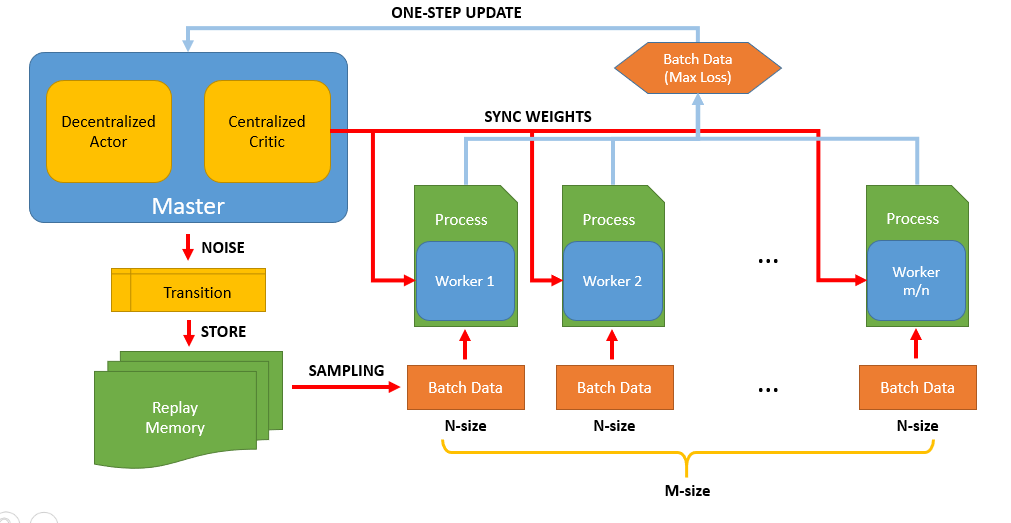
\includegraphics[width=12cm]{imgs/architecture.PNG}
  \caption{architecture}
  \label{fig:architecture}
 \end{center}
\end{figure*}

\section{Proposed Methods}[on-going]
We have discussed in previous sections that traditional reinforcement learning methods perform poorly in our multi-agent domain environment. In this section, we will introduce our proposed method: Distributed Multi-Agent DDPG. The method could be split into two part. One is the Multi-Worker using threading programming. And another one is that we use clipping method to prevent traning from slow learing and over-fitting.
[Some constrains or obvious advantage of our proposed method]

\subsection{Distributed Multi-Agent DDPG}
Recently, OpenAI rleased a method which extends traditional DDPG method to multi-agent domain \cite{maddpg}. As we know, single-agent algorithm failed because while agent is updating policy, the environment becomes non-stationary which turns out to failure of convergence. \textbf{Multi-Agent DDPG} found a centralized way to put other agents's actions into consideration in critic.
\begin{equation}
L(\theta_i) = E_{s,a,r,s'}[(Q^*(s, a_1, a_2 ... a_n) - y)^2],  
\end{equation}
$$where\ y = r_i + \gamma{Q_i}^*(s', a_1', a_2' ... a_n') | _{a_j'=\mu_j'(o_j)}$$
This is a great iead to learn using centralized critic and act using decentralized actor. 

Based on the centralized critic idea from MADDPG, we introduce our two approaches towards multi-agent task in Predator-Prey environment. \par

In traditional DRL methods like DQN or DDPG, we use replay memory to solve the problem that there are close connections between transitions. When training, add transition into repley memory, then when updating network, sample batches from replay memory with a fixed size. However, along with the network updating, old experiences seems less meaningful for learning comparing with batches which were gotten from recent policy. 
In our Distributed method, we use $\mathbb{N}$ workers to work for us, in charge of collecting batch data. Each worker runs on different threading with same environment (different random noise for each worker), collection (state, actions, rewards, done, next state) then pushing into a fixed-size memory. When memory is full, our brain starts to update using this batch data using the two equation in MADDPG. Because we have different work working on parallel world, correlation problem between batch data is solved in our method. \ par
Also we adopt target network idea. The target netowork keeps frozen (dont change parameters) for a period of time. The policy network uses it to calculate the TD errors.

\subsection{Policy Optimization by clipping}
Although Policy gradient methods are foundamental break-through using Deep Neural Network, it is difficult to obstain good result using policy gradient methods because it is extremely sensetive about choosing learning step size. If iteration step size is too small, training will be very slow; if it is too large, training process will be influenced by noise which turns out to a poor performance and over-fitted result. \par
Proximal Policy Optimization (PPO) \cite{ppo} is the method which gets inspiration from Trust Region Policy Optimization and does a well trade-off among implementation simplicity, Sample complexity and Tuning difficulty. PPO tries to calculate a update in every iteration step to minimize lost function and ensures a small deviation compared with previous policy when calculating gradient.


\begin{algorithm*}
\caption{Distributed Worker on each thread Algorithm}
\begin{algorithmic}
\State {Initialize a random process $\mathbb{N}$ for action exploration}
\State {Receive initial state $s$}
\For {$t = 1$ to max-episode-length}
  \State {for each agent $i$, select action $a_i = \pi_i(o_i) + \mathbb{N}_t$ w.r.t the current policy and exploration}
  \State {Execute actions $a = (a_1 ... a_n)$ and observe reward $r = (r_1 ... r_n)$ for each agent and new state $s'$}
  \If {Queue size is not equal to max-batch-size}
    \State {Store $(s, a, r, s')$ in Queue which could be accessed by other thread}
  \EndIf
\EndFor
\end{algorithmic}
\end{algorithm*}

\begin{algorithm*}
\caption{Distributed Multi-Agent Cooperation Algorithm based action-value function}
\begin{algorithmic}
\State {Initiate brain and n workers for n agents}
\State {}
\For {$episode = 1$ to M}
  \State {}
  \For {$t = 1$ to max-episode-length}
    \State {Get batch data $(s, a, r, s')$ from Queue}
  \EndFor
\EndFor
\While {$queue \neq empty$}   
    \State $node1 \gets queue.pop()$
    \State {$node1\ mark\ as\ "abstracted"$}
    \If {node1 has no unabstracted neighbor}
        \State {Abstract node1 as (level+1) node to new Graph with node1's position}
        \State {$Continue$}
    \EndIf
    \State {$node2 \gets node1's\ unabstracted\ neighbor$}
    \State {Abstract node1, node2 as (level+1) node to new Graph with node1 and node2's average position}
    \State {Push node1, node2's unabstracted neighbor to queue}
\EndWhile
\Return {$new graph$}
\end{algorithmic}
\end{algorithm*}

\section{Empirical Experiments}
In this section, we will introduce the experiment environment we use and several experiment we carried to verify the superiority of our proposed method.
\subsection{Experiment Environment}
To perform our experiments, we adopt the multiagent-particle-envs used in \cite{maddpg}, which consists of $N$ agents and $L$ landmarks inhabiting a two-dimensional world with continuous space and discrete time. There are several types of environment it provides with, according to our goal, we focus on Predator-Prey environment.
\begin{figure}[ht]
 \begin{center}
  \includegraphics[width=5cm]{imgs/adversary_chasing.png}
  \caption{Adversary Chasing}\label{fig:adversaryChasing}
 \end{center}
\end{figure}
In this Predator-Prey environment, $N$ slower cooperating agents must chase the faster target which could flee away from chasers around a randomly generated environment with $L$ large landmarks served as obstacles to blcok the way. Each time agents collide with a target, the agens are rewarded while the target is penalized. \par
Due to being short of calculation capability and resources, we add some constrains in Predator-Prey environment.
\begin{itemize}
  \item $N$ Predators, $\subseteq$ $[2, 4]$ with random initial position.
  \item $M$ Preys, $\subseteq$ $[1, 2]$ with random initial position.
  \item $1$ Landmark, with a fixed position in middle.
\end{itemize}
The action space is Box(5) in gym [reference]
\begin{table}[ht]
 \caption{action space} 
 \label{tbl:action}
  \begin{center}
    \begin{tabular}{c|ccc}
  Num  & Action & Min & Max\\
  \hline \hline
  0 & No use &  & \\
  1 & Power toward right & -1.0 & 1.0\\
  2 & Power toward left & -1.0 & 1.0\\
  3 & Power toward up & -1.0 & 1.0\\
  4 & Power toward down & -1.0 & 1.0\\\hline
    \end{tabular}
  \end{center}
\end{table}
The observation space is Box($6+N*2$) for each chaser and Box($4+N*2$) for target, which includes every agent's position and environment information.
\subsection{Network Architecure}

\begin{table}[ht]
 \caption{Hyper Parameters} 
 \label{tbl:hyperparameters}
  \begin{center}
    \begin{tabular}{c|ccc}
  \hline \hline
  Actor Learning rate  & 0.001   \\
  Critic Learning rate & 0.01    \\
  Gamma                & 0.99    \\
  Replay memory size   & 1000000 \\
  Minibatch size       & 64      \\
  Max episodes         & 10000   \\
  Max episode length   & 200     \\
  Random seed          & 1234    \\\hline
    \end{tabular}
  \end{center}
\end{table}

\begin{figure}[h]
 \begin{center}
  \includegraphics[width=8cm]{imgs/actor.PNG}
  \caption{Actor Network Architecture}\label{fig:Actor}
 \end{center}
\end{figure}

\begin{figure}[h]
 \begin{center}
  \includegraphics[width=8cm]{imgs/critic.PNG}
  \caption{Critic Network Architecture}\label{fig:Critic}
 \end{center}
\end{figure}



\begin{comment}

\section{序論}
執筆要領について述べる。

\subsection{用紙}
A4用紙を縦長に使用する。本文は8ページ(表裏で4枚)以上、24ページ以内を標準とする。

\subsection{ヘッダ・フッタ}
ヘッダの左側には、「筑波大学大学院博士課程システム情報工学研究科修士論文」につづけて、修了年度・月を括弧書きで記述する。
ヘッダの右側には、氏名を記述する。氏名については、見やすくするために適宜空白をいれても差し支えない。

フッタの中央には、ページ番号をハイフンはさんで記述する。

\subsection{1ページ目の体裁}
申請する学位(修士(工学))を四角囲みで記述し、
つづけて修士論文のタイトルをそれぞれ日英表記で記述する。
ただし本文が英文の場合、英日の順に記述する。

つぎに、氏名・所属専攻と指導教員名・指導教員の所属を日英表記で記述する。
氏名・指導教員名については、見やすくするために適宜空白をいれても差し支えない。
ただし本文が英文の場合、英日の順に記述する。


\subsection{要約・キーワード}
修士論文の概要を記述する。
本文が日本語・英語に係らず概要は英語で記述する。


\subsection{本文}
本文は2段組みとし、10.5pで記述する。
句読点は、各分野で用いられる記号を使用する。

\subsection{図表}
論文として印刷に耐えうる品質(解像度)の図表を作成する。
図表中、および、キャプションは、原則として英語を使用する。
キャプションは、図の下と表の上に挿入する。
図番号および表番号は、それぞれ Figure 1、Table 1 のように表記する。
横長の図・表の場合は、段抜きで挿入してもよい。

たとえば、Figure \ref{fig:samplefigure}や Table \ref{tbl:sampletable}を例として示す。

\begin{figure}[t]
 \begin{center}
  \includegraphics{sample.eps}
  \caption{Sample figure}\label{fig:samplefigure}
 \end{center}
\end{figure}

\begin{table}
 \caption{Sample table} \label{tbl:sampletable}
\begin{center}
  \begin{tabular}{c|ccc}
  A & B & C & D\\
  \hline \hline
  a & b & c & d\\
  a & b & c & d\\ \hline
 \end{tabular}
\end{center}
\end{table}

\subsection{数式}
数式のサンプルとして、(\ref{eq:gauss})を示す。
\begin{equation}
 \int _\infty ^\infty e^{-x^2}dx = \sqrt{\pi} \label{eq:gauss}
\end{equation}

\subsection{参考文献}
それぞれの分野の記述法により、十分な数の参考文献を引用する\cite{osamu}。著者が執筆した修士論文に関連する内容の論文等がある場合には、必ず文献として引用する。

\subsection{著者紹介}
学会誌論文の一般的な著者紹介を例に記述する。

\subsection{付録}
本文には書ききれないデータなどは、
付録に収めることができる。付録は、研究室で別途保管する。



\section{\LaTeX スタイルファイルについて}
このサンプルは、筑波大学大学院システム情報工学研究科知能機能システム専攻の修士論文を\LaTeX で作成するためのスタイルファイルである。
配布ファイルは以下の通りである。
\begin{description}
 \item[iit-jp-sjis.sty]  知能機能システム専攻の修士論文のためのスタイルファイル
 \item[templete.tex] スタイルファイルを利用するためのテンプレートファイル
 \item[face.eps] 顔写真用のテスト画像
 \item[sample.eps] Figure のためのテスト画像
\end{description}

スタイルファイルやテンプレートは、適宜改良をして使用してもよい。

\section*{謝辞}
本研究は、・・・・・・深謝する。


%\addcontentsline{toc}{section}{\numberline{}参考文献}

\begin{thebibliography}{9}
\bibitem{osamu}  工学修得, ``修士論文の書き方'', 知能機能システム学会論文誌, Vol.1, No.2, pp.34--56, 2015.
\end{thebibliography}


\vspace{2zh}
\begin{minipage}{73mm}
 \begin{wrapfigure}[6]{l}[-4pt]{30mm} 
 \begin{center}
  \includegraphics[width=30mm]{face.eps}
 \end{center}
 \end{wrapfigure}
 \noindent 筑 \ 波 \ 太 \  郎\\\\
 筑波大学大学院システム情報工学研究科知能機能システム専攻所属
\end{minipage}

\vspace{3zh}
----------------------------------------------\par

\begin{itemize}
 \item Webで公開する論文の概要は、別に作成する。
 \item 修士論文は両面印刷とする。
 \item 修士論文提出時は、ソフトカバーを施して必要部数を大学院教務に提出する。背表紙は不要。
 \item 論文審査後に、両面印刷したもの(綴じていないもの)を専攻長に提出する。
 \item 専攻長は、専攻全員の修士論文をハードカバーにて製本し、専攻室で保管する。
\end{itemize}

\begin{itemize}
 \item Extended summary is also required for uploading onto the web.
 \item The thesis should be printed in double face printing.
 \item Submit your thesis to the academic service office. The thesis should be clapped with a soft-cover.
 \item  Submit your thesis to the chair of the iit, after it has passed the examining meeting. The thesis should not be clapped.
 \item The chair of the iit will bind up all the accepted theses and preserve in his/her office.
\end{itemize}
https://scholar.google.com/scholar?hl=zh-CN&as_sdt=02C5&q=policy+gradient&btnG=
\end{comment}

\begin{thebibliography}{9}

\bibitem{alphago}
David Silver, Aja Huang, Chris J Maddison, Arthur Guez, Laurent Sifre, George van den Driessche, Julian Schrittwieser, Ioannis Antonoglou, Veda Panneershelvam, Marc Lanctot, et al. Mastering the Game of Go with Deep Neural Networks and Tree Search. Nature, 529(7587):484–489, 2016.

\bibitem{alphagozero} 
David Silver, Julian Schrittwieser, Karen Simonyan, Ioannis Antonoglou, Aja Huang, Arthur Guez, Thomas Hubert, Lucas Baker, Matthew Lai, Adrian Bolton, Yutian Chen, et al. Mastering the game of Go without human knowledge. Nature, 550:354–359, 2017.

\bibitem{starcraft} 
DeepMind and Blizzard open StarCraft II as an AI research environment. https://deepmind.com/blog/deepmind-and-blizzard-open-starcraft-ii-ai-research-environment.

\bibitem{game}
 P. Peng, Q. Yuan, Y. Wen, Y. Yang, Z. Tang, H. Long, and J. Wang. \textsl{Multiagent bidirectionally-
coordinated nets for learning to play starcraft combat games}. CoRR, abs/1703.10069, 2017.

\bibitem{robot}
L. Matignon, L. Jeanpierre, A.-I. Mouaddib, et al. \textsl{Coordinated multi-robot exploration under
communication constraints using decentralized markov decision processes}. In AAAI, 2012.

\bibitem{google}
DeepMind AI reduces google data centre cooling bill by 40. https://deepmind.com/blog/deepmind-ai-reduces-google-data-centre-cooling-bill-40/.

\bibitem{maddpg} 
R Lowe, Y Wu, A Tamar, J Harb, P Abbeel, et al. \textsl{Multi-Agent Actor-Critic for Mixed Cooperative-Competitive Environments}.arXiv:1706.02275v2, 2017.

\bibitem{qlearning} 
Christopher JCH Watkins and Peter Dayan. \textsl{Q-Learning}. Machine Learning, 8(3-4):279–292, 1992.

\bibitem{pg} 
R. S. Sutton, D. A. McAllester, S. P. Singh, and Y. Mansour. \textsl{Policy gradient methods for rein-
forcement learning with function approximation}. In Advances in neural information processing systems, pages 1057–1063, 2000.

\bibitem{ddpg} 
Timothy P Lillicrap, Jonathan J Hunt, Alexander Pritzel, Nicolas Heess, Tom Erez, Yuval Tassa, David Silver, and Daan Wierstra. \textsl{Continuous Control with Deep Reinforcement Learning}. In ICLR, 2016.

\bibitem{ppo} 
John Schulman, Filip Wolski, Prafulla Dhariwal, Alec Radford,and Oleg Klimov. \textsl{Proximal Policy Optimization Algorithms}.arXiv:1707.06347, 2017.

\bibitem{cover} 
Xiao Tang, Nobuhara Hajime. \textsl{Real-time Grid-based Multi-Agent Pursuing A Moving Target method}. the 79th national convention of IPSJ, 2016. 

\bibitem{dpg} 
David Silver, Guy Lever, Nicolas Heess, Thomas Degris, Daan Wierstra, and Martin Riedmiller. \textsl{Deterministic Policy Gradient Algorithms}. In ICML, 2014.

\bibitem{dqn} 
Volodymyr Mnih, Koray Kavukcuoglu, David Silver, Andrei A Rusu, Joel Veness, Marc G Bellemare, Alex Graves, Martin Riedmiller, Andreas K Fidjeland, Georg Ostrovski, et al. \textsl{Human-Level Control through Deep Reinforcement Learning}. Nature, 518(7540):529–533, 2015.

\bibitem{replay} 
Long-Ji Lin. \textsl{Self-Improving Reactive Agents Based on Reinforcement Learning, Planning and Teaching}. Machine Learning, 8(3–4):293–321, 1992.

\bibitem{a3c} 
Volodymyr Mnih, Adria Puigdomenech Badia, Mehdi Mirza, AlexGraves, Timothy P Lillicrap, Tim Harley, David Silver, and Koray Kavukcuoglu. \textsl{Asynchronous Methods for Deep Reinforcement Learning}. In ICLR, 2016.

\bibitem{a2c} 
Jane X Wang, Zeb Kurth-Nelson, Dhruva Tirumala, Hubert Soyer, Joel Z Leibo, Rémi Munos, Charles Blundell, Dharshan Kumaran, and Matt Botvinick. \textsl{Learning to Reinforcement Learn}. In CogSci, 2017.

\end{thebibliography}

\end{document}